\documentclass{article}

% - style template
\usepackage{base}

% - title, author, etc.
\title{PHYS4004 - Assignment 4 - Workflow}
\author{Tom Ross - 1834 2884}
\date{\today}

% - headers
\pagestyle{fancy}
\fancyhf{}
\rhead{\theauthor}
\chead{}
\lhead{\thetitle}
\rfoot{\thepage}
\cfoot{}
\lfoot{}

% - document
\begin{document}

The entire code repository can be found at
\url{https://github.com/dgsaf/hpc-assignment-4}.

\tableofcontents

\listoffigures

\listoftables

\clearpage

\section{Interpretation}
\label{sec:interpretation}

The \lstinline{count} process is presented in \autoref{lst:count}.

\lstinputlisting[
label={lst:count}
, caption={
  The process \lstinline{process count} in \lilf{nextflow/main.nf}.
}
, language=
, morekeywords={process, input, output, container, shell, from, into}
, linerange={48-69}
, firstnumber=48
]{../nextflow/main.nf}

\begin{enumerate}[i.]
\item
  \lstinline[otherkeywords={>}]!echo "seed,ncores,nsrc" > results.csv!

  The output of the left hand side (SNR seed, number of cores used and number of
  sources counted) which would normally be sent to \lstinline{stdout} is
  redirected to the destination specified on the right hand side (in this case,
  a file called \lilf{results.csv}) creating/overwriting the file in the
  process.

\item
  \lstinline[otherkeywords={>>}]!echo "${seed},${cores},${nsrc}" >> results.csv!

  Similar to the effect of \lstinline[otherkeywords={>}]!>! above, except that
  this operator appends to the file, rather than overwriting it.

\item
  \lstinline[otherkeywords={|}]!cat ${f} | wc -l!

  The output of the left hand (normally send to \lstinline{stdout}) is
  \textit{piped} to input of the right hand side; that is, the input of
  \lstinline{wc -l} is taken from the output of \lstinline!cat ${f}!.
  This effect of this command is to count the number of lines in the file with
  filepath \lstinline!${f}!.

\item
  \lstinline!$(<command>)! and \lstinline!($(<command>))!

  Wrapping a shell command with a single pair of parentheses,
  \lstinline!(<command>)! executes that command in a sub-shell - prefixing this
  with a dollar sign captures the final output of that subshell
  \lstinline!$(<command>)!.
  However if the result of this is a list of whitespace-delimited strings,
  wrapping this in a further set of parentheses, \lstinline!($(<command>))!,
  will capture the output as an array variable.

\item
  \lstinline!$(ls table*.csv)!

  The effect of \lstinline!ls table*.csv! is to list all files in the current
  directory which start with \lstinline!table! and end with \lstinline!.csv!.
  The effect of \lstinline!$(ls table*.csv)! is to capture this list of matching
  files as a string.
  Specifically, it collects the files containing tables of counted sources for
  all combinations of \lstinline{seed} and \lstinline{cores}.

\item
  \lstinline!echo ${f}!

  The effect of this command is to output (to \lstinline{stdout}) the
  string-value of the variable \lstinline{f}.
  Specifically, this outputs the filepath of a specific file, which is taken
  from the list of tables described above, and will be of the form
  \lstinline!table_<seeds>_<cores>.csv!.

\item
  \lstinline!tr '_.' ' '!

  The effect of this command is, for a given input, to translate all instances
  of the characters \lstinline!_! and \lstinline!.! into whitespace.
  Specifically this transforms \lstinline!table_<seeds>_<cores>.csv! into
  \lstinline!table <seeds> <cores> csv!.

\item
  \lstinline!awk '{print $2 " " $3}'!

  The effect of this command is, for a given input consisting of lines
  (delimited by \lstinline!\n!) containing records (delimited by whitespace), to
  print the second record, followed by a white space, followed by the third
  record, for each line in the input.
  Specifically, this transforms \lstinline!table <seeds> <cores> csv! into
  \lstinline!<seeds> <cores>!.

\item
  \lstinline!cat ${f}!

  The effect of this command is to output the contents of the file, with
  filepath \lstinline!${f}! - specifically
  \lstinline!table_<seeds>_<cores>.csv!.

\item
  \lstinline!wc -l!

  The effect of this command is to, for a given input, count the number of
  newlines (occurences of \lstinline!\n!) in the input.
  Specifically, this counts the number of newlines in the file
  \lstinline!table_<seeds>_<cores>.csv!.

\item
  \lstinline!echo "$(cat ${f} | wc -l)-1" | bc -l!

  The effect of this command is to count the number of sources in the file
  \lstinline!table_<seeds>_<cores>.csv!, by first counting the number of lines
  in the file, and then subtracting for the number of lines which are not source
  data records.

% \item
%   remove this \lstinline!cat ${f}!

\end{enumerate}

\clearpage

\section{Development}
\label{sec:development}

\lstinputlisting[
label={lst:count}
, caption={
  The channel \lstinline{counted_ch} is duplicated, with one for each of
  \lstinline{process plot_for}, and \lstinline{process plot_xargs}, in
  \lilf{nextflow/main.nf}.
}
, language=
, morekeywords={process, input, output, container, shell, from, into}
, linerange={72-72}
, firstnumber=72
]{../nextflow/main.nf}

\subsection{Bash For Loop}
\label{sec:bash-for-loop}

\lstinputlisting[
label={lst:count}
, caption={
  The process \lstinline{process plot_for} in \lilf{nextflow/main.nf}.
}
, language=
, morekeywords={process, input, output, container, shell, from, into}
, linerange={75-93}
, firstnumber=75
]{../nextflow/main.nf}

\subsection{xargs Command}
\label{sec:xargs-command}

\lstinputlisting[
label={lst:count}
, caption={
  The process \lstinline{process plot_for} in \lilf{nextflow/main.nf}.
}
, language=
, morekeywords={process, input, output, container, shell, from, into}
, linerange={96-113}
, firstnumber=96
]{../nextflow/main.nf}

\section{Execution}
\label{sec:execution}

\subsection{SNR Plot}
\label{sec:snr-plot}

\begin{figure}[h]
  \centering
  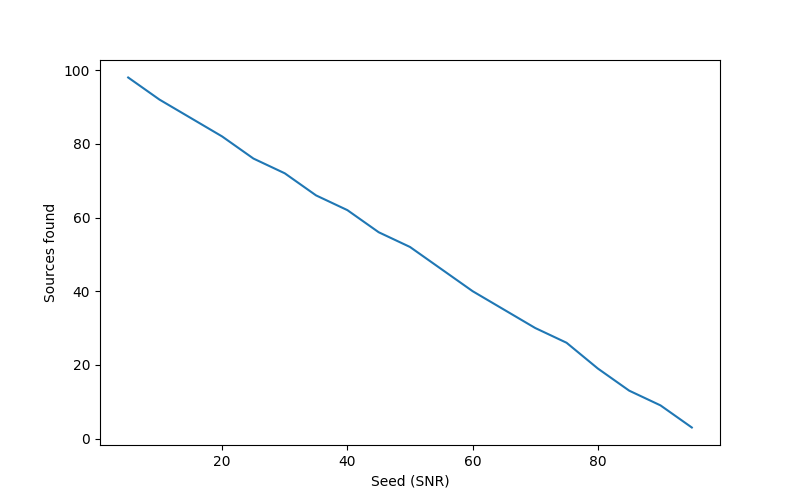
\includegraphics[scale = 0.75]{../nextflow/output/plot_for_1.png}
  \caption[SNR Plot]{
    The Signal-to-Noise Ratio (SNR) is presented for a range of seed SNR values.
    This figure was produced by
    \lstinline[morekeywords={process}]{process plot_for}, for the case of
    \lstinline{cores = 1}.
    No difference was observed between this plot and any of the other plots
    produced for any value of \lstinline{cores}, nor whether if
    \lstinline[morekeywords={process}]{process plot_for} or if
    \lstinline[morekeywords={process}]{process plot_xargs} were used.
  }
  \label{fig:snr-plot}
\end{figure}

\subsection{Workflow DAG}
\label{sec:workflow-dag}

\begin{figure}[h]
  \centering
  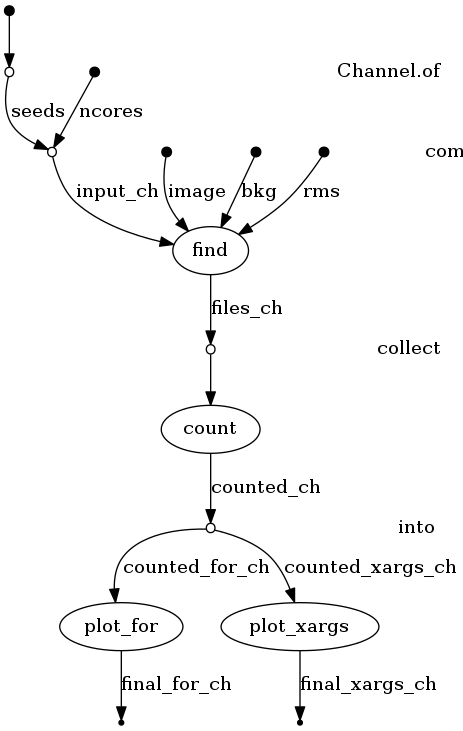
\includegraphics[scale = 0.4]{../nextflow/logs/final_dag.png}
  \caption[Workflow DAG]{
    The Directed Acyclic Graph (DAG) of the workflow is presented.
    Note that the \lstinline{combine} operator (below \lstinline{Channel.of})
    appears to have been cropped out by the tool producing the DAG.
  }
  \label{fig:workflow-dag}
\end{figure}

\clearpage

\section{Analysis}
\label{sec:analysis}

\end{document}
